\chapter{Related Work}

This chapter reviews the previous works related to this thesis on the adaptation of transformer and BERT with adapters in machine translation. Specifically, in \cref{sec:prelm_mt}, we review works in incorporating BERT for machine translation. In \cref{sec:adapter_seq}, we review the usage of adapters using transformer as the base model in sequence to sequence models in various fields such as NLU, Automatic Speech Recognition (ASR), and MT.

\section{Pre-training Language Models in Machine Translation}
\label{sec:prelm_mt}

This section will discuss three different works that try to incorporate BERT into NMT. The goals of these works are different from the experiments proposed in this thesis because they are primarily leveraging the feature representation of BERT instead of using BERT directly to fine-tune NMT.

\normcite{weng2020acquiring} propose to acquire knowledge from pre-trained models such as BERT with a framework called $A_{PT}$. $A_{PT}$ consist of two different modules with different goals. The first goal is to learn a task-specific representation through adaptation from general representation in the pre-trained models and to learn two controlling methods to control the task-specific representation into NMT. They propose to achieve the first goal by using a dynamic fusion mechanism. They claim this method could provide rich contextual information to model sentences in NMT better. An illustration of their proposed approach can be seen in \cref{img:dyn_fn}. The second goal is via knowledge distillation to prune the knowledge from pre-trained models. They claim this method could help NMT to continuously learn essential knowledge about translation from source sentence to target sentence by using parallel data and help generate better translation by learning from monolingual data. Moreover, based on their empirical results, they achieve the best results when both the methods are applied in the encoder and decoder. We refer to \cref{img:kdweng} for illustration of this approach.

\begin{figure}[h]
    {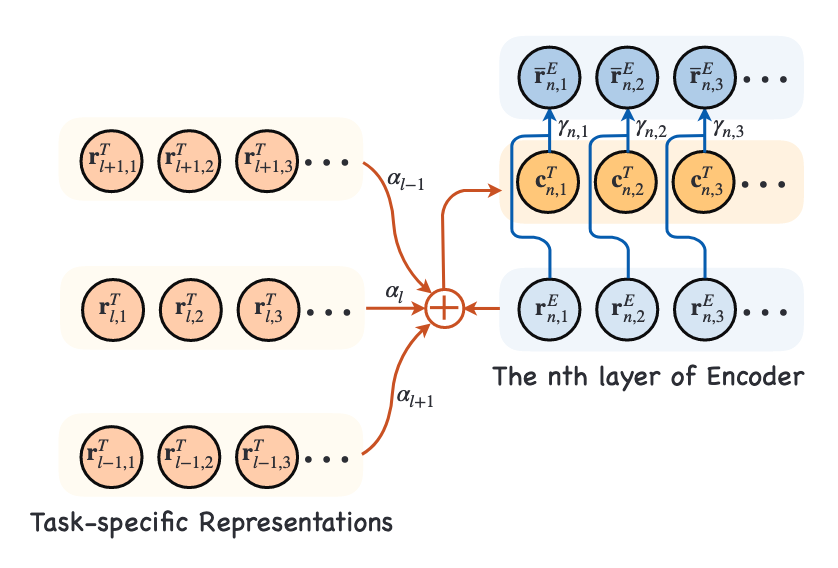
\includegraphics[width=0.75\textwidth]{img/dynamic_fusion.png}}
    \centering
    \caption{Illustration of dynamic fusion mechanism. Figure reprinted from \normcite{weng2020acquiring}.}
    \label{img:dyn_fn}
\end{figure}

\begin{figure}[h]
    {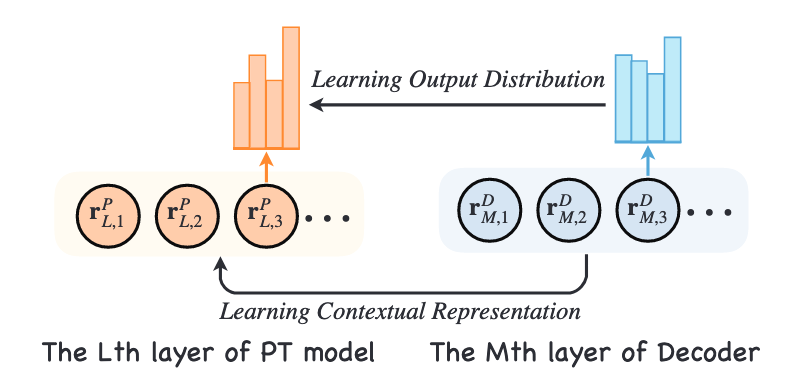
\includegraphics[width=0.85\textwidth]{img/kdweng.png}}
    \centering
    \caption{Illustration of knowledge distillation mechanism. Figure reprinted from \normcite{weng2020acquiring}.}
    \label{img:kdweng}
\end{figure}

\normcite{yang2020towards} try to combat issues such as requiring a long time to train NMT models and catastrophic forgetting problem from updating too many of the pre-trained models in the fine-tuning process. They propose a concerted training approach ($CT_{NMT}$) that consists of three different techniques: 1) Asymptotic distillation; 2) Dynamic switch for knowledge fusion; 3) Rate-scheduled updating. The first technique is used to keep the pre-trained knowledge intact. They achieve this by using the pre-trained BERT as a teacher network and the encoder of the NMT models as the student. The goal of the first technique is to mimic the representation coming from the pre-trained BERT by minimizing the cross-entropy loss. The second technique is introduced to perform a combination between the representation from BERT and the encoder of NMT. They achieve this by using a gating mechanism that uses the source as the input to decide how to fuse the representations. The intuition of this technique is that for a particular sentence, BERT might provide a better representation than the currently trained model. Using this gating mechanism, they try to adjust the use of BERT representation in the encoder dynamically. The intuition of this gating mechanism is that BERT might better encode some sentences but not all. The last technique uses a scheduling policy for adjusting the learning rate. They propose using this as they found that updating BERT LM and the NMT at different paces would benefit the final model. An illustration of the asymptotic distillation and dynamic switch mechanism is depicted in Figure \ref{img:ctnmt}.

\begin{figure}[h]
    {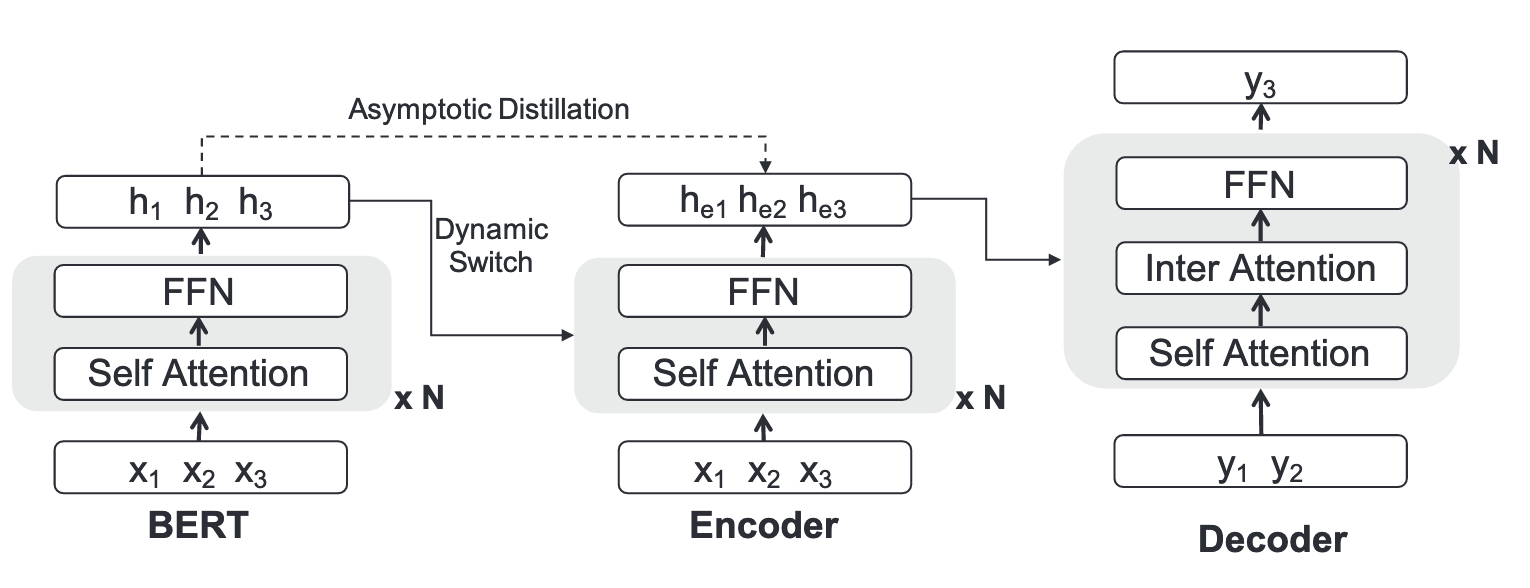
\includegraphics[width=0.95\textwidth]{img/ctnmt.png}}
    \centering
    \caption{Illustration of asymptotic distillation and dynamic switch. Figure reprinted from \normcite{yang2020towards}.}
    \label{img:ctnmt}
\end{figure}

\normcite{chen2019distilling} notices the discrepancy between the objective used to pre-train BERT and the objective used in common NLG tasks such as MT. They propose to introduce knowledge distillation approach learned in BERT for text generation tasks. The first proposal introduces a new objective called Conditional Masked Language Modeling (C-MLM). This objective is inspired by MLM but induces another conditional constraint while fine-tuning the pre-trained BERT on a target dataset. The second approach consist of leveraging the fine-tuned BERT as a teacher model and using the logits output as the learning target for the student network to mimic. They claim that the proposed approach improves the generation output as they now leveraging BERT's bidirectional ability to \textit{plan ahead}. They also claim that BERT's ability to look forward into the future can act as an effective regularizer that can help to boost the quality of the generated output.

\begin{figure}[h]
    {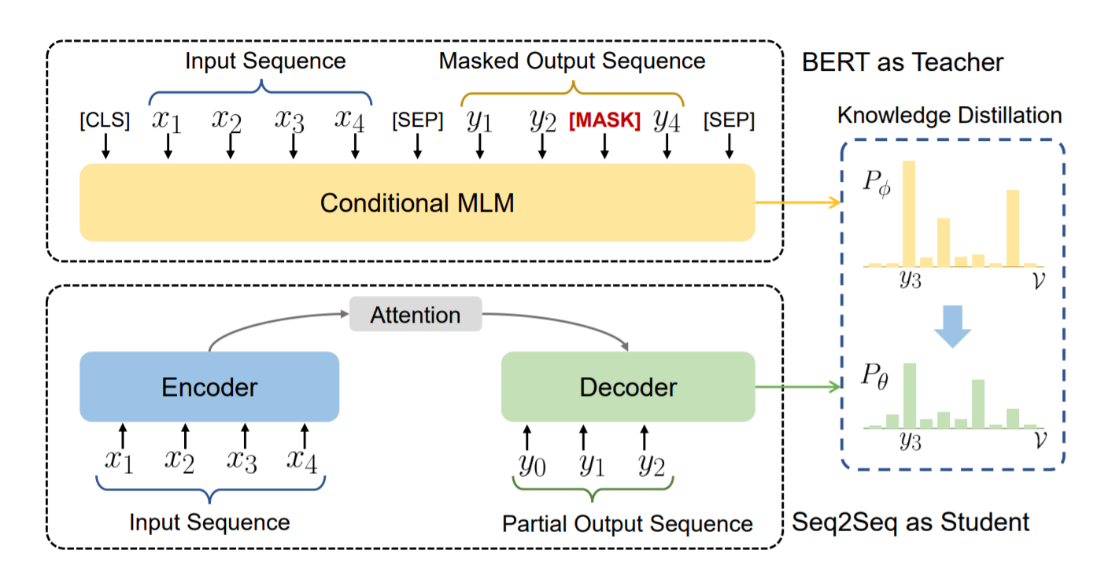
\includegraphics[width=0.95\textwidth]{img/bert_distill.png}}
    \centering
    \caption{Illustration of seq2seq architecture. Figure reprinted from \normcite{chen2019distilling}.}
    \label{img:bert_distill}
\end{figure}

\section{Adapters in Sequence-to-Sequence}
\label{sec:adapter_seq}

In this section, we divide the discussions and reviews into three areas. \cref{sec:adapter_place} discusses the importance of adapters placement in the transformer layers as well as in the sequence to sequence framework. The first part reviews the work of \normcite{houlsby2019parameter} and \normcite{bapna2019simple}. Both works propose the same concept of adapters with similar architecture. The difference between them lies in the placement of the adapters within the transformer layer. The other work by \normcite{winata2020adapt} discuss the importance of adapters in sequence-to-sequence framework. They found interesting results where adapters in encoder have more impact than in the decoder.

\cref{sec:app_nlu_asr} and \cref{sec:app_mt} review the application of adapters in other fields such as NLU and ASR as well as in the machine translation. Each will discuss the type of adapters used, the purpose of the adapters, and the impact of including the adapters as a part of their training procedure.

\subsection{Placement of Adapters}
\label{sec:adapter_place}
There are two types of adapters placement in the transformer architecture. The first type of adapter was proposed by \normcite{houlsby2019parameter}. We recall that each transformer layer consisted of two sub-layers: a self-attention layer and a feedforward layer. Each sub-layers will be followed immediately by a projection layer whose job is to transform the feature's size back to the original input size. The adapters are applied to the output of the sub-layer of the transformer. Specifically, it is applied to the output of the projection layer that transforms the vectors back to the input size and before being applied to the skip connection. The illustration of the adapter architecture can be seen in Figure \ref{img:ada_houlsby}.

\begin{figure}[h]
    {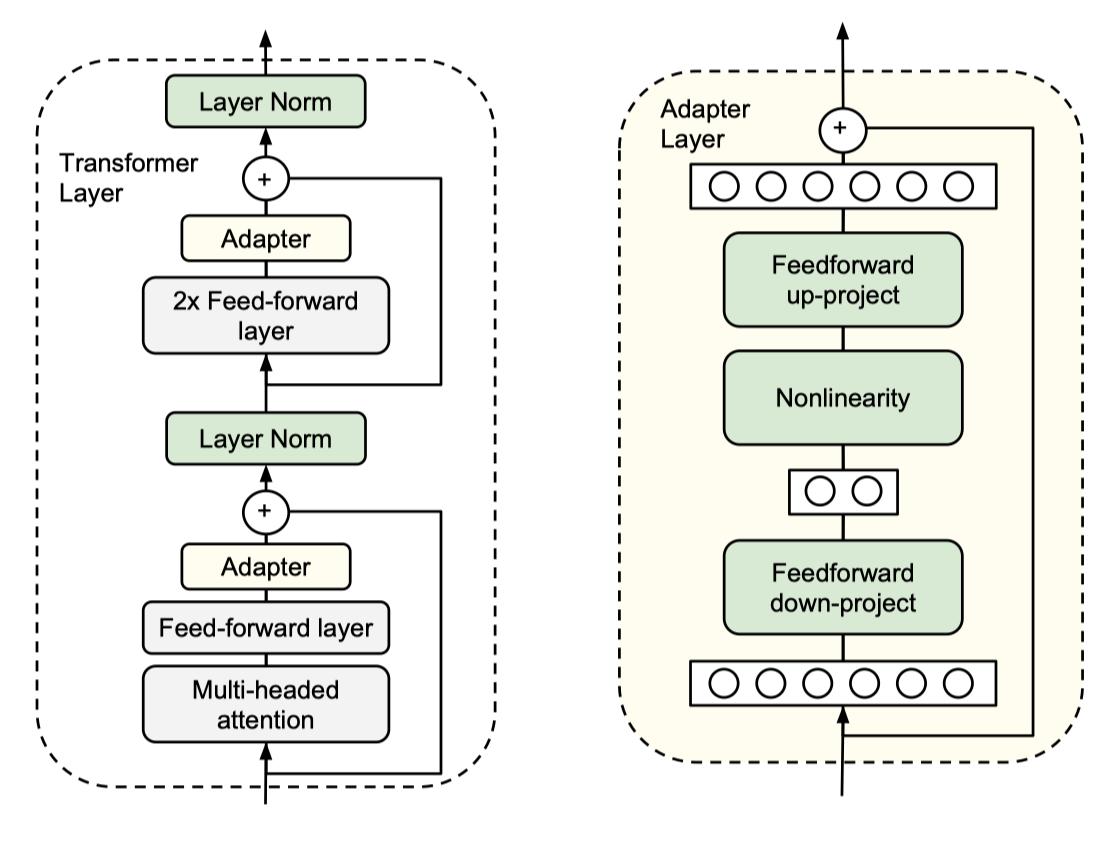
\includegraphics[width=0.95\textwidth]{img/adapter_houlsby.png}}
    \centering
    \caption{Illustration of adapter architecture. Figure reprinted from \normcite{houlsby2019parameter}.}
    \label{img:ada_houlsby}
\end{figure}

The second work of adapters is published by \normcite{bapna2019simple}. They take a simpler approach in contrast to \normcite{houlsby2019parameter} in regards to incorporating the adapters into the transformer network. Rather than inserting two serial adapters into the sub-layers of the transformer, they instantiate a single instance of adapters and place it on the top of each layer. In addition to the simpler design of adapter layers, they add layer normalization to normalize the input of the adapters. The reasoning behind this is to make the adapters pluggable into any part of the base networks, ignoring the distribution variations of the previous layers. For illustration we refer to Figure \ref{img:ada_bapna}.

\begin{figure}[h]
    {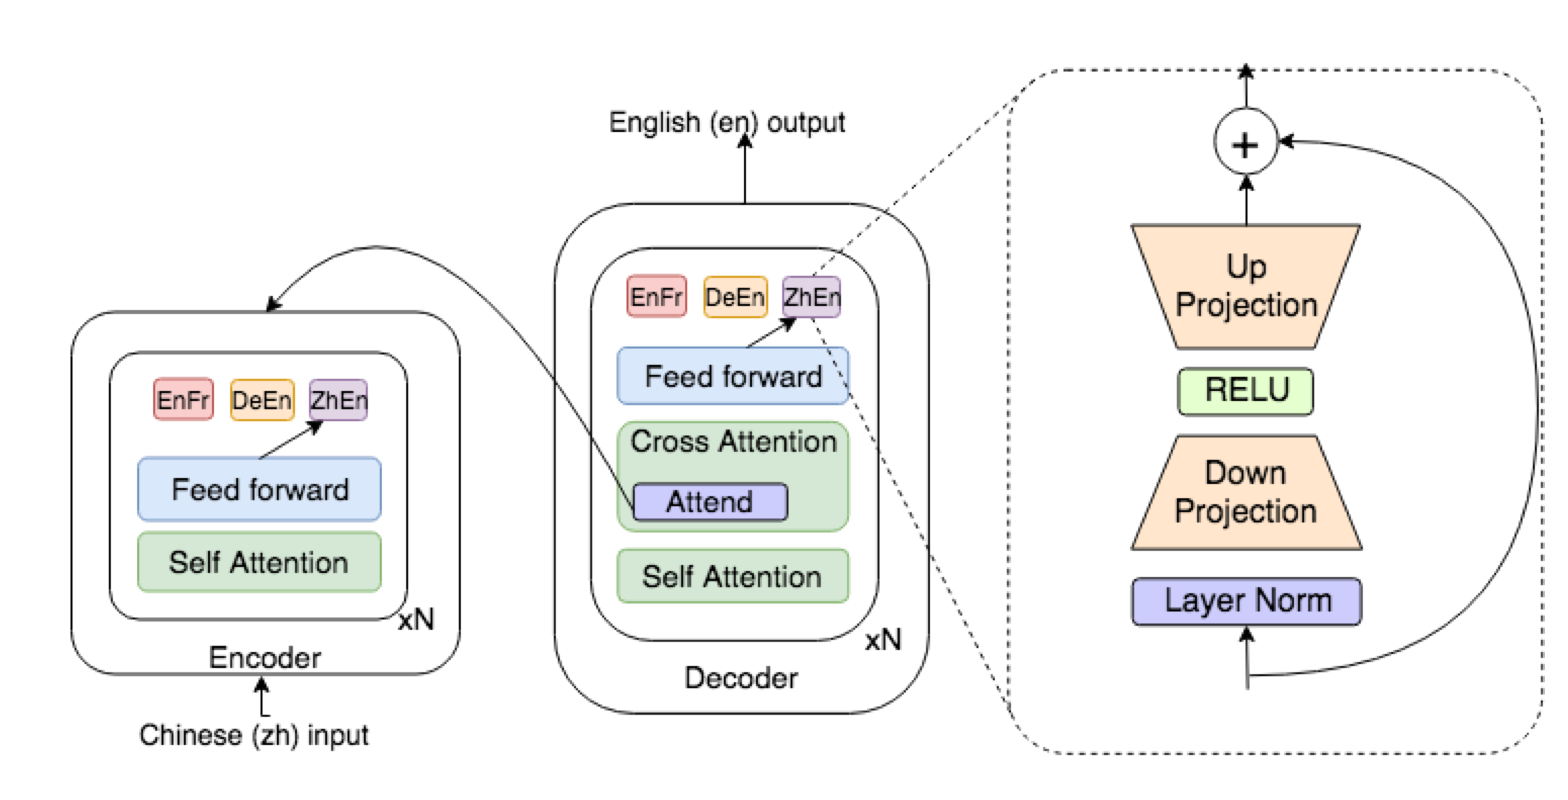
\includegraphics[width=0.95\textwidth]{img/adapter_bapna.png}}
    \centering
    \caption{Illustration of adapter architecture. Figure reprinted from \normcite{bapna2019simple}.}
    \label{img:ada_bapna}
\end{figure}

\normcite{pfeiffer2021adapterfusion} mentioned that the placement of adapter parameters within a pre-trained model is non-trivial and thus requires extensive experiments. To identify the best setup for the placement of the adapter, the authors perform an exhaustive search on the hyperparameters. This includes the position and the number of adapters within a single layer, the position of residual connections, the bottleneck residual factors, as well as the non-linearity within the bottleneck adapter layer. In their experiments that involve both NLU and NLG, they find the best performing adapter is close to the simple architecture proposed by \normcite{bapna2019simple} and not from \normcite{houlsby2019parameter}.

We now discuss the placement of the adapters from the perspective of the encoder-decoder framework (sequence-to-sequence). \normcite{winata2020adapt} conducted an experiment using similar adapter architecture and placement to \normcite{bapna2019simple} in ASR. The encoder in this work represents a model whose job is to encode audio representation. The decoder is responsible for encoding the text features and generating text output. In this work, the authors perform experiments comparing the effectiveness of adapters in both encoder and decoder. They initialized the decoder using pre-trained mBERT weights \normcite{devlin2018bert}. Based on their findings, adapters in the decoder are not as effective as they are in the encoder component. These results indicate that adapting the weights in the audio space is more effective for the model's performance than in the text space. Features in mBERT may have already provided enough good features so that further fine-tuning may no longer be necessary.

\subsection{Adapters in NLU and Automatic Speech Recognition}
\label{sec:app_nlu_asr}
Adapters have been used as an alternative for naive fine-tuning in various fields in NLP. \normcite{houlsby2019parameter} introduces adapters to fine-tune BERT model in various NLU tasks. Primarily, they use the adapters in GLUE \citewithpar{wang2018glue} and additional classification tasks. They conducted another experiment on a more complicated problem such as SQuAD \citewithpar{rajpurkar2018know}. They found positive results in using adapters in GLUE, other classification, and SQuAD tasks compared to naive fine-tuning. By adding a small number of parameters, they achieved a comparable performance in all tasks compared to fine-tuning the whole weights. We can refer to \cref{sec:adapter_place} for the explanation and illustration of the adapters architecture of their work.

\normcite{pfeiffer2020madx} experiments with adapters involve bootstrapping pre-trained NLP models such as BERT, and XLM \citewithpar{conneau2019cross} in low-resource languages. They perform two types of adaptation, language-adaptation and task-adaptation. For this purpose, they use two different adapters in different situations. The language-adapters are trained with the MLM objective to capture various features in different languages. They then put task adapters on top of the language adapters for further fine-tuning for each of the tasks in their experiments. They use an efficient adapter architecture based on \normcite{pfeiffer2021adapterfusion} which has similarities to the work of \normcite{bapna2019simple}. For more details on the architecture definition, we refer the reader to \cref{sec:adapter_place}. They perform their experiments on three different tasks: Named Entity Recognition (NER), extractive question answering (QA), and causal commonsense reasoning (CCR). These tasks are available in multilingula test sets that cover both high-resource and low-resource languages. We refer the reader to their original paper for more details on the dataset they used on each task. Their main finding is that the task-specific adapters perform similarly to the work of \normcite{houlsby2019parameter}. However, since their main focus is on multilingual setup, they did not find satisfying results due to low output quality in unseen languages. With the help of language adapters, they have improved the performance across all tasks. The performance is especially appealing in low-resource languages.

\normcite{winata2020adapt} evaluate adapters performance in multilingual ASR setup. They use a similar setup as \normcite{bapna2019simple} to adapt both the encoder and decoder. They employ adapters to combat language mismatch and improve models' robustness in various languages with limited resources. Their main finding for the adapters is that it improves the performance across various languages. Furthermore, they also performed experiments to generate a cluster of languages where similar languages are put within the same group. They then share the adapters to languages belonging to the same group and find out that this helps performance in low-resource languages but has small drawbacks in the high resource languages.

\normcite{lee2021adaptable} propose multi-domain adapters for language model in ASR setup. Specifically, they employ the adapters in the language model (LM) component for rescoring purposes in an ASR system. They use the similar architecture of the adapter to the work of \normcite{houlsby2019parameter} where they introduce adapters within the sub-networks as well as at the top of the layer. Their experiments show that by using separate adapters for each domain, they can re-use a general domain LM and switch domains by replacing adapters with the one that has already been fine-tuned on the respective domain. They also found that with the help of adapters, they manage to improve the performance on a specific problem, such as predicting proper nouns.

\subsection{Adapters in Machine Translation}
\label{sec:app_mt}
\normcite{bapna2019simple} propose an alternative to \normcite{houlsby2019parameter}. Instead of using two different adapters within a single transformer layer, they propose to use a single adapter on top of the layer. Another difference is that they add layer normalization after the transformer layer output. Furthermore, they also experiment with the adapters in the NLG domain instead of NLU. They use machine translation objective for the pre-training objective and treat the adapters as the adaptation module for a specific language pair. They first pre-trained the model in a large parallel corpus such as WMT before performing domain adaptation on a smaller corpus such as IWSLT in the same language pair. In a single language pair experiment, they found out that the architecture of the proposed adapter is flexible with respect to the size of the data when the adapter's capacity is properly adjusted to match the requirements for the corpus size adaptation. Furthermore, they found out that they did not find any sign of overfitting; instead, they found the model to reach its peak and stay steady throughout the training process.

\normcite{philip2020monolingual} apply adapters in multilingual machine translation differently than \normcite{bapna2019simple}. \normcite{bapna2019simple} use adapters for every target pair. For example, in the English French pair, they have to create two different adapters for English$\rightarrow$French and French$\rightarrow$English. \normcite{philip2020monolingual} propose to use a monolingual adapter where instead of using a single adapter for a language pair, they use a single adapter for each of the languages. They use the same adapter architecture as in \normcite{bapna2019simple}. Their findings suggest that their approach reduced the number of adapters from $n(n-1)$ to $2n$. Furthermore, they also find that this approach has better performance in low-resource languages than the one proposed in \normcite{bapna2019simple}.

\normcite{guo2021adaptive} show that adding adapters to BERT during the fine-tuning can be beneficial in the machine translation task. The purpose of the adapters in this work is to make the fine-tuning process more lightweight than the regular fine-tuning. They follow the adapter architecture and use a similar mechanism to include the adapters on the base model as \normcite{bapna2019simple}. The difference is that \normcite{bapna2019simple} do not use BERT as the base model and use a plain transformer that is pre-trained using machine translation objective.

% The difficulties of incorporating BERT in machine translation has already explained in \ref{sec:domain_adapt}. \cite{guo2021adaptive} also propose that


% \section{Fine-tuning in Sequence-to-Sequence Framework}